\label{Zustand}

Damit der genaue Ablauf unseres Programms definiert ist, wurde mithilfe von Enterprise Architect das Zustandsdiagramm aus Abbildung \ref{fig:Statemachine} gezeichnet. \\
Auf unser Projekt übertragen bedeutet es, dass das Diagramm vom Einschalten der Hardware, durch Stromversorgung des Arduinos, über jede Kombinationsmöglichkeiten der Taster, bis hin zum wieder Ausschalten der Hardware, alle Zustände zeigt, in welche das Programm kommen kann. Dies soll später dem Softwareentwickler die Arbeit vereinfachen. Des Weiteren können auch Tests mithilfe des Zustandsdiagramms leichter durchgeführt werden, da die Eingangsvariablen mit den darauffolgenden Zustandsänderungen, eindeutig zu erkennen sind. \\

\begin{figure}[!hbt]
	\centering
	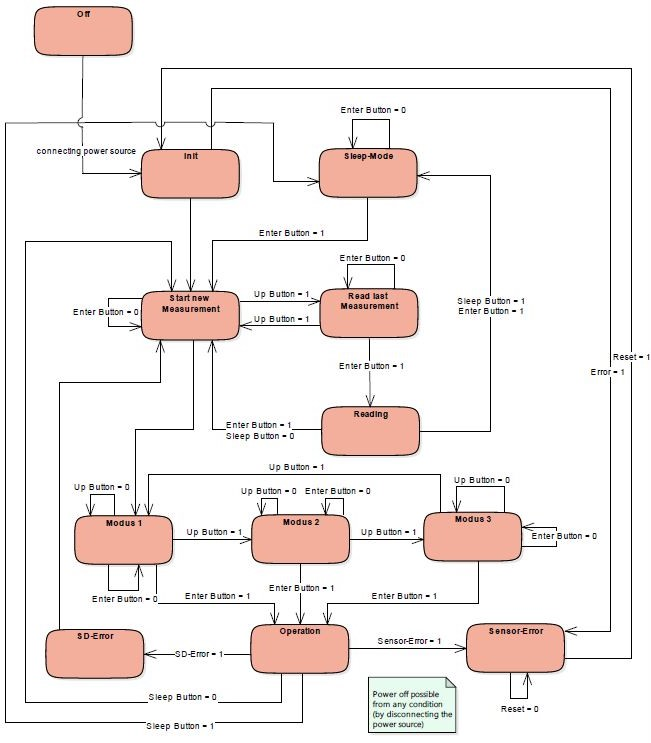
\includegraphics[width=0.9\linewidth]{Images/Statemachine}
	\caption{Entwurf des Zustandsdiagramms mithilfe von Enterprise Architect}
	\label{fig:Statemachine}
\end{figure}
